%llncs    article
\documentclass[a4paper,parskip=full-]{article}

\usepackage{amsmath}
\usepackage{amssymb}

\usepackage{tikz}
\usetikzlibrary{decorations.pathreplacing}

\usepackage{graphicx}  % images
%\usepackage{qtree} % for trees
\usepackage{lmodern}  %THE tex font :)
\usepackage{url}  %urls in references
%\usepackage{prettyref}
%\usepackage{pstricks} %graphicv2
\usepackage{cite}
\usepackage{enumerate}
\usepackage{multicol}
\usepackage{xspace}
\usepackage{color}
\usepackage{algorithmic} 
\usepackage{wasysym}
\usepackage[ngerman]{babel}
\usepackage[utf8]{inputenc} % Zeichenkodierung   utf8   latin1
%\include{biblio} % references
\usepackage{listings}                           % for source code inclusion
\usepackage{multirow} 
\usepackage{caption}
\usepackage{wrapfig}
%absatz
\usepackage{setspace} 

%breaking math formulars automaticly
%http://tex.stackexchange.com/questions/3782/how-can-i-split-an-equation-over-two-lines
\usepackage{breqn}

%Durchstreichungen
%\cancel
%http://de.wikibooks.org/wiki/LaTeX-Kompendium:_F%C3%BCr_Mathematiker#Durchstreichungen
\usepackage{cancel}

%Für Römische Zahlen
\usepackage{enumitem}
%\usepackage{romannum}%stdclsdv

%Durchstreicen möglich
\usepackage[normalem]{ulem}

%Bessere Brüche
\usepackage{nicefrac}

%bookmarks
%\usepackage[pdftex,bookmarks=true]{hyperref}
%[pdftex,bookmarks=true,bookmarksopen,bookmarksdepth=2]
\usepackage{hyperref}
%\usepackage{scrhack}

%fußnoten
\usepackage{footnote}
\usepackage{caption} 

\usepackage{geometry}
\geometry{verbose,a4paper,tmargin=25mm,bmargin=25mm,lmargin=15mm,rmargin=20mm}

%randnotiz
\newcommand\mpar[1]{\marginpar {\flushleft\sffamily\small #1}}
\setlength{\marginparwidth}{3cm}

%svg Grafiken
%http://tex.stackexchange.com/questions/122871/include-svg-images-with-the-svg-package
\usepackage{svg}

%http://tex.stackexchange.com/questions/48653/making-subsections-be-numbered-with-a-b-c
\usepackage{chngcntr}
\counterwithin{subsection}{section}

%Sektions nicht Nummerrrieren (<=> section*{...})
% \makeatletter
% \renewcommand\@seccntformat[1]{}
% \makeatother
\setcounter{secnumdepth}{0}

\title{Machine Learning \\
Exercise sheet 3}

\author{Gruppe 9: \\Hauke Wree and Fridtjof Schulte Steinberg}

\newcommand{\R}[0]{{\mathbb{R}}}

\newcommand{\N}[0]{{\mathbb{N}}}
\newcommand{\C}[0]{{\mathbb{C}}}
\newcommand{\K}[0]{{\mathbb{K}}}
\newcommand{\lF}[0]{{\mathcal{l}}}
\newcommand{\I}[0]{{\mathcal{I}}}
\newcommand{\nhnh}[0]{{\frac{n}{2} \times \frac{n}{2}}} %nice
\newcommand{\norm}[1]{\left\lVert#1\right\rVert}
%\newcommand{\rm}[1]{\romannumeral #1}
\newcommand{\RM}[1]{\MakeUppercase{\romannumeral #1{.}}} 

\renewcommand \thesubsection{\alph{subsection}}

\begin{document}

\maketitle

\section{Exercise 1 (Linear support vector machines – “toy” example):}

\subsection{a)}

Da $\vec{w}^T \cdot \vec{x}^{(\text{test1})} = b^*$

%\subsection{b)}

%Die umkreisten Datenpunkte $\vec{x}^{(\mu)}$ %$ \vec{x)^{(\mu)} $%  ,y^{(\mu)} )$, %mit $y^{\mu} \cdot \left( \vec{w}^T  \cdot \vec{x)^{\mu} + b\right) = 1$, 
werden \textit{Support Vektoren} genannt. 
\section{Exercise 3 (Nonlinear SVM – XOR-problem to illustrate the kernel trick)}
Sei 
$\Phi : \R^2 \rightarrow \R^6, \begin{pmatrix} x_1 \\ x_2 \end{pmatrix} \mapsto 
\begin{pmatrix} x_1^2 \\ x_2^2 \\ \sqrt{2} x_1 \\ \sqrt{2} x_2 \\ \sqrt{2} x_1 x_2 \\ 1 \end{pmatrix}$

\subsection{a)}
$$
\Phi(x)^T \cdot \Phi(y) = 
\begin{pmatrix} 
x_1^2 & x_2^2 & \sqrt{2} x_1 & \sqrt{2} x_2 & \sqrt{2} x_1 x_2 & 1 
\end{pmatrix} 
\cdot \begin{pmatrix} y_1^2 \\ y_2^2 \\ \sqrt{2} y_1 \\ \sqrt{2} y_2 \\ \sqrt{2} y_1 y_2 \\ 1 \end{pmatrix}
= x_1^2 \cdot y_1^2 + x_2^2 \cdot y_2^2 + 2 x_1 y_1 + 2 x_2 y_2 + 2 x_1 x_2 y_1 y_2 + 1
$$

\subsection{b)}

Sei die Kernelfunktion $k$ gegeben mit:
\begin{dmath}
k(\vec{x}^T \cdot \vec{y}) = (\vec{x}^T \cdot \vec{y})
= (\vec{x}^T \cdot \vec{y})^2 + 2(\vec{x}^T \cdot \vec{y}) + 1
= x_1^2 \cdot y_1^2 + x_2^2  \cdot y_2^2 + 
\sqrt{2} x_1  \cdot  \sqrt{2} y_1 + \sqrt{2} x_2  \cdot  \sqrt{2} y_2 +
\sqrt{2} x_1 x_2  \cdot  \sqrt{2} y_1 y_2 + 1 \cdot 1 = \begin{pmatrix} 
x_1^2 & x_2^2 & \sqrt{2} x_1 & \sqrt{2} x_2 & \sqrt{2} x_1 x_2 & 1 
\end{pmatrix} 
\cdot \begin{pmatrix} y_1^2 \\ y_2^2 \\ \sqrt{2} y_1 \\ \sqrt{2} y_2 \\ \sqrt{2} y_1 y_2 \\ 1 \end{pmatrix}
= \Phi(x)^T \cdot \Phi(y)
\end{dmath}

\subsection{c)}
\begin{tabular}{|c|c|c|c|}
%\caption{XOR}
\hline
$x_1$ & $x_2$ & xor($x_1$, $x_2$) & $\Phi(x_1,x_2)$ \\
\hline \hline
-1 & -1 & -1 & $
\begin{pmatrix}
 1 &
 1 &
 -\sqrt{2} &
 -\sqrt{2} &
 \sqrt{2} &
 1 
\end{pmatrix}^T$ \\
\hline
-1 & 1 & 1 & $\begin{pmatrix}
 1 &
 1 &
 -\sqrt{2} &
 \sqrt{2} &
 -\sqrt{2} &
 1 
\end{pmatrix}^T$ \\
\hline
1 & -1 & 1 & $\begin{pmatrix}
 1 &
 1 &
 \sqrt{2} &
 -\sqrt{2} &
 -\sqrt{2} &
 1 
\end{pmatrix}^T$ \\
\hline
1 & 1 & -1 & $\begin{pmatrix}
 1 &
 1 &
 \sqrt{2} &
 \sqrt{2} &
 \sqrt{2} &
 1 
\end{pmatrix}^T$ \\
\hline
\label{tab:xor}
\end{tabular}

Da für die 4 Möglichen Eingaben $\{-1,1\}^2$ die Ausgabe für $\Phi$ sich nur in 3 Dimensionen unterscheiden, können wir diese als 3D-Punkte darstellen. 

%\begin{figure}
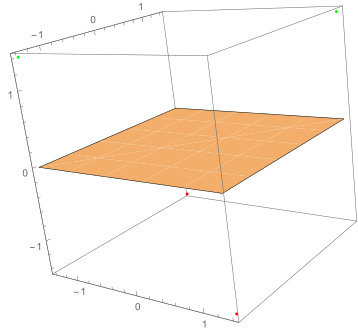
\includegraphics[scale=1]{3c}
%\input{3c.pdf_tex}
%\end{figure}



\end{document}